% ============================================================
% SECTION: Molecular Docking
% ============================================================
\section{Molecular Docking}

\begin{frame}{AutoDock Vina: Molecule Preparation}
  \begin{columns}[T]
    \begin{column}{0.52\textwidth}
      \begin{block}{Ligand Preparation}
        \begin{enumerate}
          \item SMILES $\rightarrow$ 3D conformer (RDKit ETKDGv3)
          \item Force-field minimisation (MMFF94)
          \item PDBQT conversion (Open Babel \texttt{-{}-gen3d})
        \end{enumerate}
      \end{block}
    \end{column}
    \begin{column}{0.45\textwidth}
      \begin{block}{Receptor Preparation}
        \begin{enumerate}
          \item Structure fetch: AlphaFold $\rightarrow$ RCSB PDB
          \item PDBQT conversion (Open Babel \texttt{-xr})
          \item Binding box (BioPython):
                \begin{itemize}
                  \item HETATM ligand centroid if co-crystal present
                  \item Protein geometric centroid otherwise
                  \item $+$ 10\,\AA\ padding, capped at 30\,\AA
                \end{itemize}
        \end{enumerate}
      \end{block}
    \end{column}
  \end{columns}
\end{frame}

\begin{frame}{AutoDock Vina: Scoring \& Search}
  \begin{columns}[T]
    \begin{column}{0.52\textwidth}
      \begin{block}{Vina Scoring Function}
        Combines empirical energy terms:
        \begin{itemize}
          \item Steric (Gaussian) repulsion/attraction
          \item H-bond energy
          \item Hydrophobic contacts
          \item Torsional entropy penalty
        \end{itemize}
        \vspace{0.15cm}
        Output: $\Delta G_{\text{bind}}$ (kcal/mol)\\
        More negative $=$ tighter predicted binding.\\
        \vspace{0.1cm}
        \small $\Delta G \leq -9$ kcal/mol $\approx$ low-nM $K_d$
      \end{block}
    \end{column}
    \begin{column}{0.45\textwidth}
      \begin{exampleblock}{Search Parameters}
        \begin{description}
          \item[Exhaustiveness] 8 (default Monte Carlo steps)
          \item[Poses] Up to 5 per ligand
          \item[Box size] 22.5\,\AA\ (co-crystal) or adaptive (centroid fallback)
        \end{description}
      \end{exampleblock}
      \vspace{0.3cm}
      \begin{alertblock}{Limitation}
        Vina scores correlate with experimental $K_d$ in
        benchmarks but are a scoring approximation, not
        a thermodynamic calculation. False positives occur,
        especially with AlphaFold receptors.
      \end{alertblock}
    \end{column}
  \end{columns}
\end{frame}

\begin{frame}{Docking Results}
  \begin{center}
    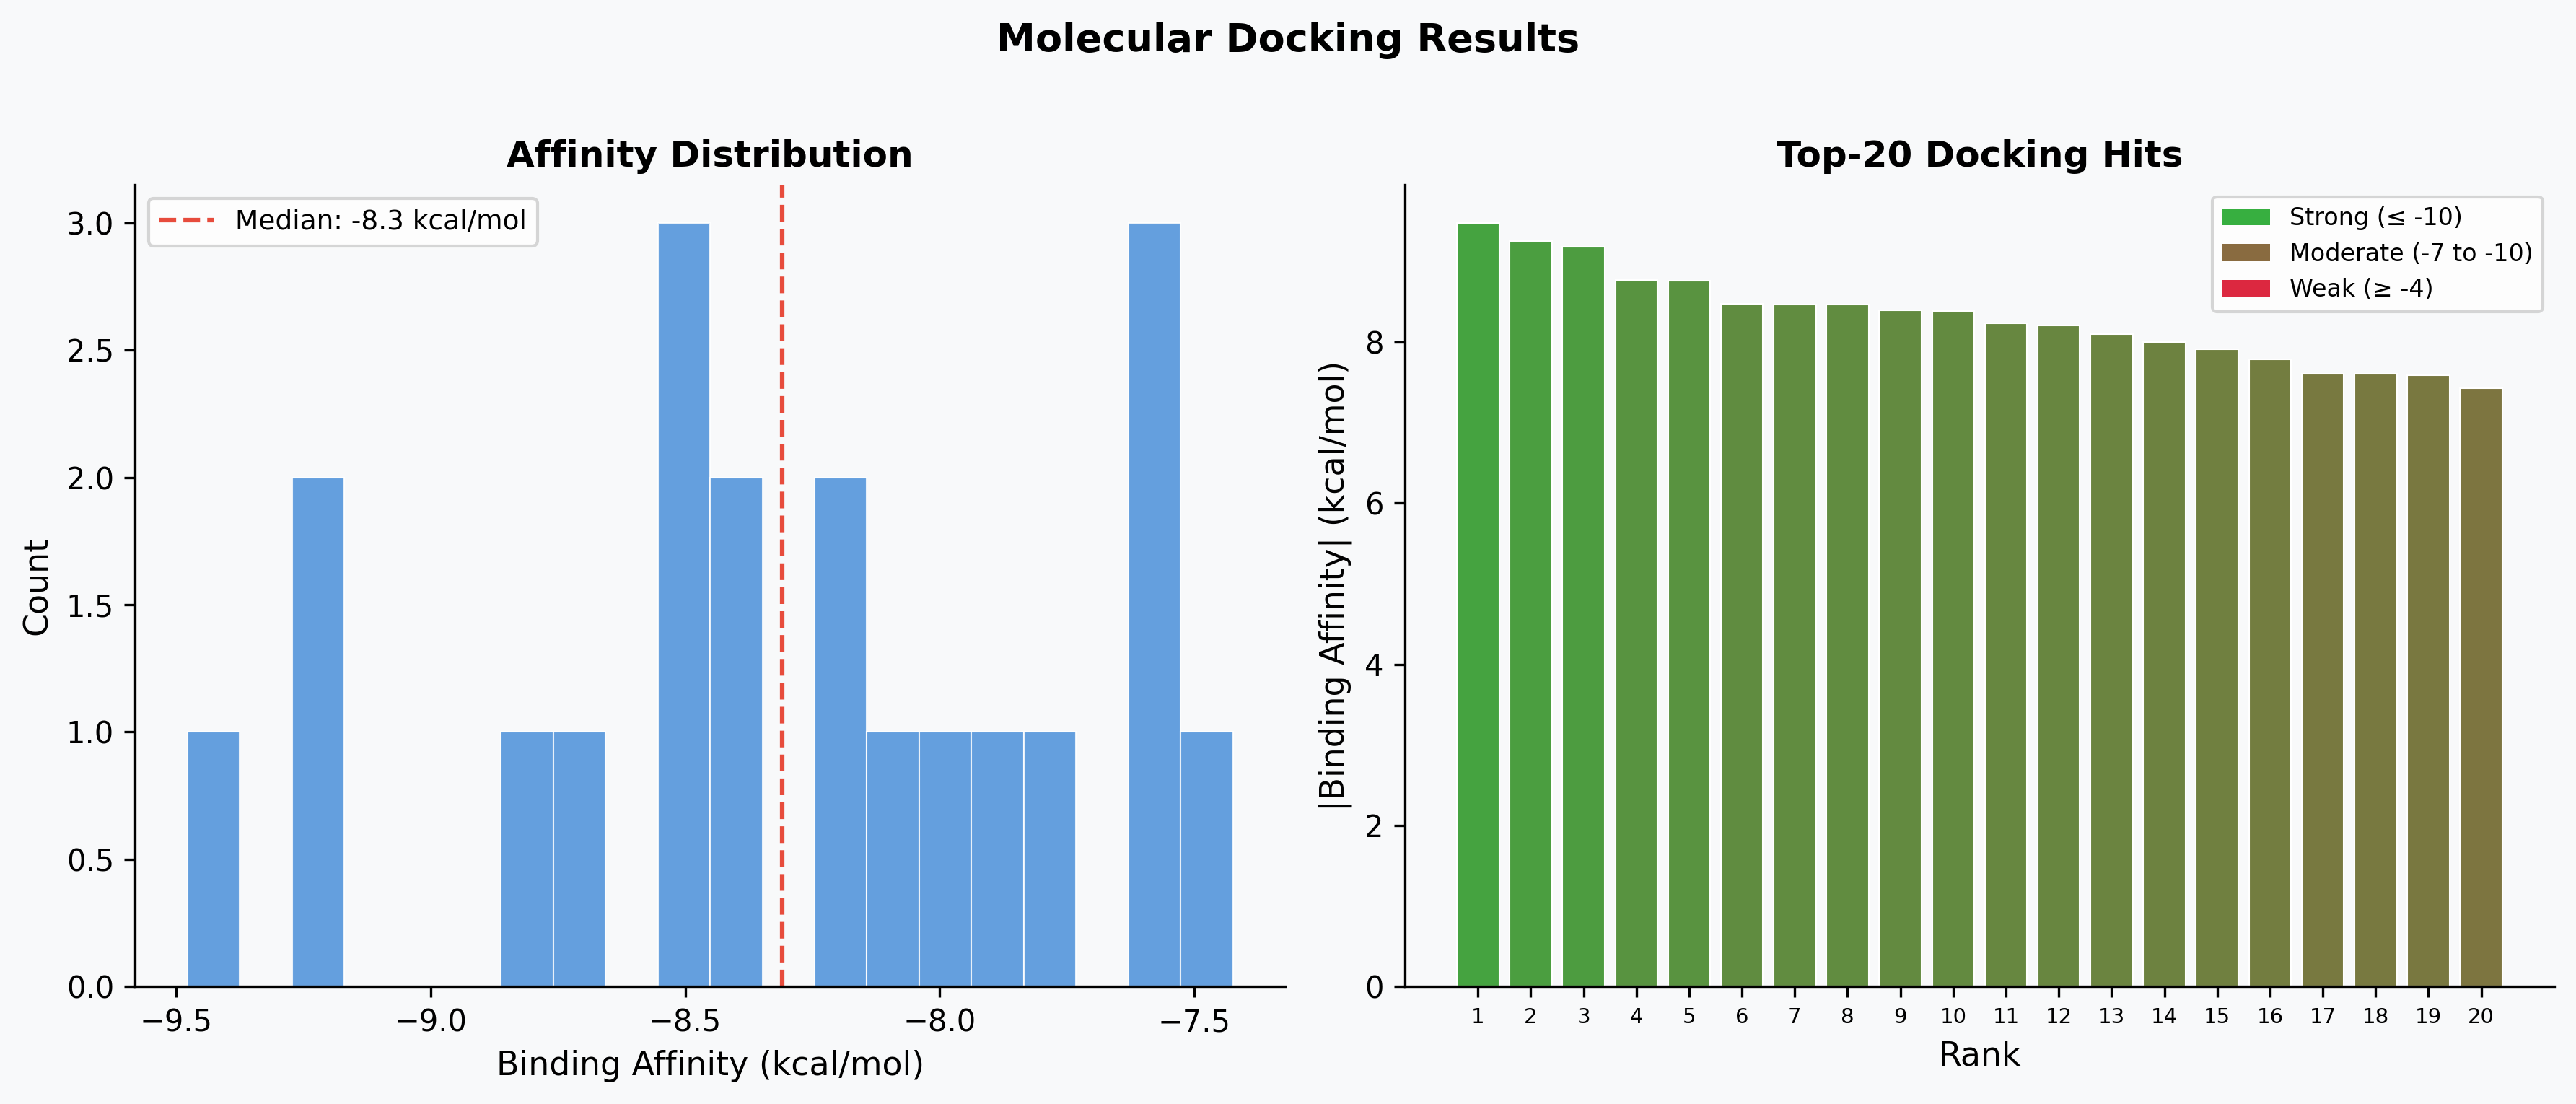
\includegraphics[width=0.88\textwidth]{../figs/docking_scores.png}
  \end{center}
  \textit{Left}: binding affinity distribution across top-20 candidates.
  \textit{Right}: ranked hits coloured by binding strength
  (green $\leq -9$\,kcal/mol, yellow moderate, red $\geq -6$\,kcal/mol).
  CDK2 — best: $-9.5$\,kcal/mol, median: $-8.2$\,kcal/mol, 3/20 below $-9$.
\end{frame}
